\documentclass[../rapport.tex]{subfiles}

\begin{document}
    \chapter{Le stage}
    \section{Sujet}
        Durant mon stage, j'ai eu l'occasion de travailler sur 3 projets successif.
        Cette alternance de projet m'a permis d'avoir des methodes de travails variées,
        et de ne pas me limiter à une seule technologie.

        J'ai eu ainsi l'occasion de travailler avec par exemple Symfony,
        Laravel, NodeJS, Docker, Typescript, RabbitMQ, MongoDB et MySQL.

        \subsection{Premier projet}
        Le premier projet sur lequel j'ai eu l'occasion de travailler visait à
        développer une application permettant de trouver du travail. Cette
        application destinée au marché asiatique était similaire à jobteaser ou
        linkedin. Je suis arrivé à la fin du développement de ce projet, et j'ai du 
        ajouter des fonctionnalité à l'\gls{api}. Celà à représenté environ un quart de mon
        stage.

        \subsection{Deuxième projet}
        Une fois le premier projet fini, j'ai été assigné à un projet de
        réécriture de micro service. 
        Le projet était commandé par SITA, et il fallait reconcevoir l'implémentation
        de certains micro services sur un de leur projet porté sur les objets
        connectés.
        Ce projet a été l'occasion pour moi de travailler en autonomie, et il a
        constitué également un quart de mon stage.

        \subsection{Troisième projet}
        Le troisième projet consistait à developper une application permettant
        de faciliter la mise en relation de voisin pour tout type de service, comme
        le baby sitting, les course, etc. Pour cette application j'ai dû travailler en
        équipe avec un autre stagiaire, ce projet a donc été pour nous de développer 
        nos compétences collaboratives afin de réaliser cette application.
    \section{Role}
        Dans ces trois projets, j'ai endossé le rôle de développeur côté
        serveur. C'est à dire que je me suis occupé du traitement des données,
        leur stockage, leur validation et le controle de leurs accès etc.
    \section{Déroulement}
        \subsection{Jobigo}
        Au tout début de mon stage, j'ai été assigné à un projet déjà en cours: Jobigo. l'objectif de
        ce projet était de permettre de trouver du travail plus facilement
        en mettant en relation chercheur d'emploi, et employeurs.
        Le projet était quasiment terminé au moment où je suis arrivé, il s'agissait simplement d'ajouter
        les derniers détails pour que l'\gls{api} puisse interagir avec l'application mobile
        de façon optimale.
        Pendant Ce projet, je me suis principalement occupé de mettre en place les \glspl{push}.
        Je n'avais pas de connaissances concernants les \glspl{push}, il a donc fallu que 
        j'apprenne en autonomie le principe de fonctionnement, avec notamment l'enregistrement 
        des \glspl{token}. On peut trouver deux types de \glspl{token}: ceux de Apple, et de Google.
        Ceux de apple sont par exemple plus compliqué à utiliser car ils nécessitent la génération 
        de certificats.

            L'api de jobigo a été principalement construite en utilisant php, avec \textit{Api platform}\footnote{https://api-platform.com/} un \gls{framework} permettant de simplifier la conception des \gls{api}.

        \subsection{Smart ULD}
        Une fois ce projet livré, j'ai été assigné à un autre projet.
        Le client en question développe un projet permettant de suivre des container
        à bord des avions, et notamment suivre leur geolocalisation.
        Pour que ce flux de données soit correctement acheminé, une architecture à base de micro-services
        avait déjà été prototypée par le client. Le but pour Siclo était donc à
        partir du prototype, de 
        redévelopper un ensemble de micro-service un peu plus robustes. Un
        résumé de l'architecture est disponible figure~\ref{fig:overview}.

        \begin{figure}
            \centering
            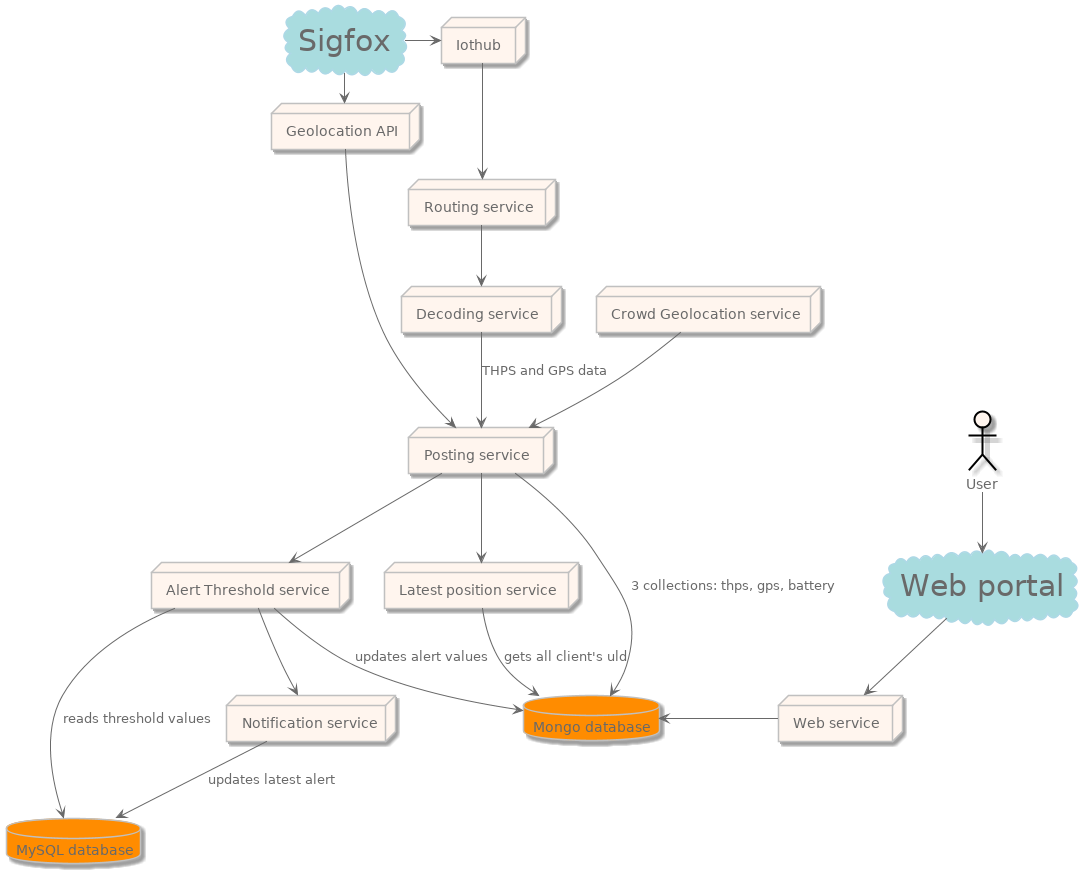
\includegraphics[scale=0.4]{servicesOverview}
            \caption{Plan de l'architecture}
            \label{fig:overview}
        \end{figure}


\end{document}
